\chapter{Estadística de la medida química}\label{ch:b2:measurement-statistics}

Dos laboratorios miden el plomo de la misma agua del grifo e informan de 9.6 y \qty{11.2}{\micro g/L}.
El valor guía para el agua de consumo es \qty{10}{\micro g/L}. ¿Es potable el agua? ¿Discrepan siquiera los dos
laboratorios, o ambos resultados son el mismo valor visto a través de la dispersión de dos
medidas? Un número procedente de un análisis no significa nada sin su incertidumbre, y este capítulo da
las herramientas para calcularla: la estadística de las medidas repetidas, la propagación de las incertidumbres
a través de un cálculo, el calibrado por mínimos cuadrados y los límites por debajo de los cuales un método no ve nada.
% ledger: who:lead

\begin{omfigure}
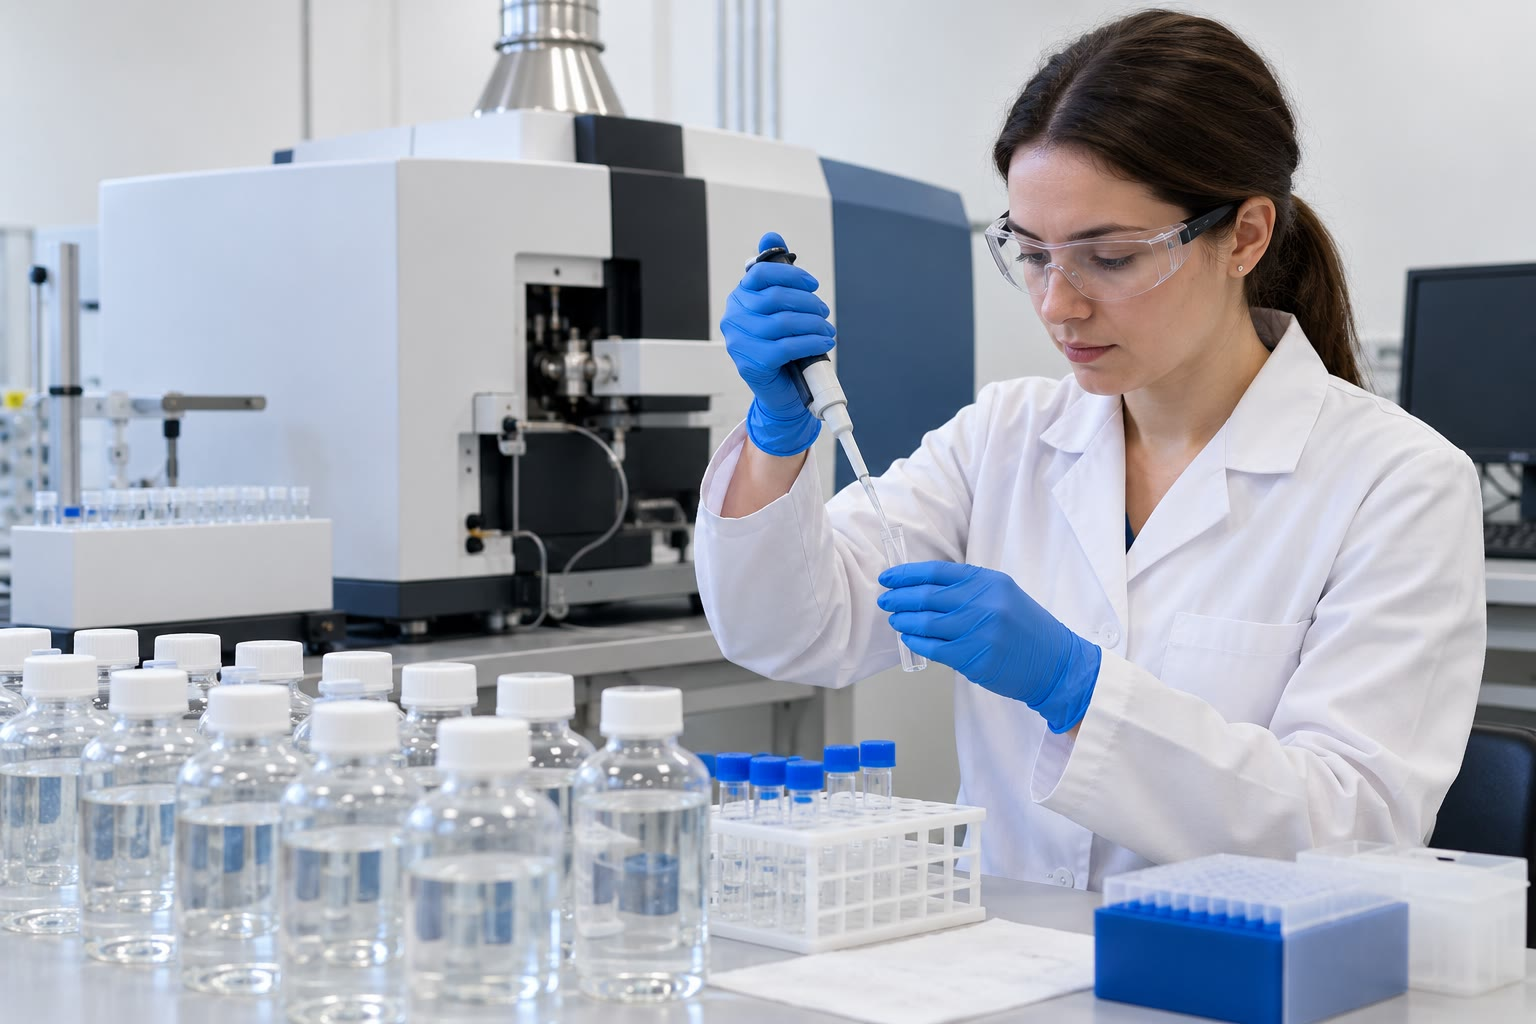
\includegraphics[width=0.56\linewidth]{images/book3/ai/b2-34-water-lab.jpg}

{\small Un laboratorio de análisis de aguas: botellas de muestra, una técnica pipeteando, un analizador elemental
al fondo (ilustración).}
\end{omfigure}

\begin{recall}
El volumen del primer año: incertidumbre de medida, incertidumbre típica, evaluaciones de tipo A y de tipo B,
incertidumbre expandida, incertidumbre relativa, desviación normalizada $z$ entre dos valores, y la
promesa de una demostración de $u(\bar x) = s/\sqrt n$ y de una regla general de propagación. El volumen escolar: la
recta de calibrado. \Cref{ch:b2:mass-spec-atomic}: la absorción atómica.
\end{recall}

\section{Medidas repetidas}

Si se repite una medida, los resultados se dispersan. Tratamos cada resultado $x_i$ como una variable aleatoria de
media $\mu$ (el valor que daría el método en promedio) y desviación típica $\sigma$; cuando se suman muchas
causas pequeñas e independientes, los resultados siguen la ley normal (gaussiana), con alrededor del 68~\% de ellos
dentro de $\mu \pm \sigma$ y el 95~\% dentro de $\mu \pm 1.96\sigma$.

\begin{definition}[Dispersión]\label{def:b2:measurement-statistics:dispersion}
Para $n$ resultados $x_1, \dots, x_n$ de media $\bar x$, la \emph{desviación típica
experimental}\index{desviacion tipica experimental@desviación típica experimental} es $s = \sqrt{\sum (x_i - \bar x)^2/(n-1)}$; es una
estimación de $\sigma$. La \emph{desviación típica de la media}\index{desviacion tipica de la media@desviación típica de la media} es
la desviación típica de $\bar x$ sobre muchas series de $n$ resultados, estimada por $s/\sqrt n$.
\end{definition}

El divisor $n - 1$ en lugar de $n$ corrige el hecho de que las desviaciones se toman respecto a $\bar x$,
calculada a su vez con los mismos datos, lo que las hace un poco demasiado pequeñas: $n - 1$ es el número de
desviaciones independientes, los grados de libertad.

\begin{theorem}[Varianza de la media]\label{thm:b2:measurement-statistics:mean-variance}
Si $x_1, \dots, x_n$ son independientes, cada uno de varianza $\sigma^2$, entonces $\operatorname{var}(\bar x) =
\sigma^2/n$: la \omterm{def:b2:measurement-statistics:dispersion}{desviación típica de la media} es $\sigma/\sqrt n$.
\end{theorem}

\begin{proof}
Para variables independientes la varianza de una suma es la suma de las varianzas, y
$\operatorname{var}(cX) = c^2\operatorname{var}(X)$. Así, $\operatorname{var}(\bar x) =
\operatorname{var}\bigl(\tfrac1n\sum x_i\bigr) = \tfrac{1}{n^2}\sum\operatorname{var}(x_i) =
\tfrac{1}{n^2}\,n\sigma^2 = \sigma^2/n$. Sustituir $\sigma$ por su estimación $s$ da la incertidumbre
típica de tipo A $u(\bar x) = s/\sqrt n$ admitida en el volumen del primer año.
\end{proof}

\section{Intervalos de confianza}

\begin{definition}[Intervalo de confianza]\label{def:b2:measurement-statistics:confidence}
Un \emph{intervalo de confianza}\index{intervalo de confianza} con un \emph{nivel de confianza}\index{nivel de confianza}
$1 - \alpha$ (a menudo el 95~\%) es un intervalo calculado a partir de los datos mediante una regla que, aplicada a
muchas series, contiene el valor verdadero en una fracción $1 - \alpha$ de ellas. Para la media de $n$ resultados
es $\bar x \pm t\,s/\sqrt n$, donde $t$ es el \emph{coeficiente de Student}\index{coeficiente de Student}
para $n - 1$ grados de libertad y ese nivel.
\end{definition}

\begin{proposition}[Ley de Student]\label{prop:b2:measurement-statistics:student}
Para $n$ resultados normales independientes, $T = (\bar x - \mu)/(s/\sqrt n)$ sigue la ley de Student con
$n - 1$ grados de libertad, cuya densidad es proporcional a $(1 + t^2/\nu)^{-(\nu+1)/2}$ con
$\nu = n - 1$. Es más ancha que la ley normal y tiende a ella cuando $n$ crece.
\end{proposition}

\admitted

Dividir por $s$ en lugar de por el desconocido $\sigma$ añade la dispersión del propio $s$, que es grande cuando $n$ es
pequeño; de ahí las colas más pesadas y los coeficientes mayores que 1.96. La tabla da los coeficientes al 95~\%,
calculados a partir de la densidad.

\begin{omfigure}
\begin{minipage}[c]{0.56\linewidth}
\begin{tikzpicture}
\begin{axis}[width=\linewidth, height=4.8cm, xmin=-5, xmax=5, ymin=0, ymax=0.43,
  xlabel={$t$}, ylabel={densidad}, label style={font=\small}, tick label style={font=\scriptsize},
  legend style={font=\scriptsize, at={(0.98,0.98)}, anchor=north east}, legend cell align=left]
\addplot[omThm, thick] table[x=t, y=nu2] {figdata/out/bachelor-2-regression-c.dat};
\addplot[omMeth, thick] table[x=t, y=nu5] {figdata/out/bachelor-2-regression-c.dat};
\addplot[black, thick, dashed] table[x=t, y=normal] {figdata/out/bachelor-2-regression-c.dat};
\legend{$\nu = 2$, $\nu = 5$, normal}
\end{axis}
\end{tikzpicture}
\end{minipage}\hfill
\begin{minipage}[c]{0.4\linewidth}\centering
\small
\begin{tabular}{rr}
\hline
$\nu = n - 1$ & $t$ (95~\%) \\
\hline
1 & 12.706 \\
2 & 4.303 \\
3 & 3.182 \\
4 & 2.776 \\
5 & 2.571 \\
9 & 2.262 \\
20 & 2.086 \\
$\infty$ & 1.960 \\
\hline
\end{tabular}
\end{minipage}
\par\vspace{4pt}

{\small Densidades de Student para 2 y 5 grados de libertad frente a la ley normal, y los coeficientes bilaterales
al 95~\%, calculados integrando la densidad (la última fila es la ley normal).}
% figdata: bachelor-2/regression.py parts c, e
\end{omfigure}

\begin{method}[Un intervalo de confianza para una media]\label{met:b2:measurement-statistics:confidence-interval}
\begin{enumerate}
  \item Calcúlense $\bar x$ y $s$ de los $n$ resultados; compruébese que ningún resultado se aparta groseramente de los demás.
  \item Léase $t$ para $\nu = n - 1$ al nivel elegido.
  \item Exprésese $\bar x \pm t\,s/\sqrt n$, con la incertidumbre redondeada a una o dos cifras significativas
        y la media a la misma posición decimal.
  \item Para comparar con un valor de referencia $x_{\mathrm{ref}}$, calcúlese $|\bar x - x_{\mathrm{ref}}|/(s/\sqrt
        n)$: por encima de $t$, la diferencia es significativa a ese nivel; por debajo, los datos no muestran
        diferencia (lo que no demuestra que no la haya).
\end{enumerate}
\end{method}

\section{Propagación de la incertidumbre}

\begin{theorem}[Ley de propagación de la incertidumbre]\label{thm:b2:measurement-statistics:propagation}
Si $y = f(x_1, \dots, x_n)$, donde las $x_i$ son independientes con incertidumbres típicas $u(x_i)$ lo bastante pequeñas
para que $f$ sea casi lineal en ellas, entonces
\begin{equation*}
u^2(y) = \sum_{i=1}^{n}\left(\frac{\partial f}{\partial x_i}\right)^2 u^2(x_i).
\end{equation*}
\end{theorem}

\begin{proof}
A primer orden (Taylor), $y - f(\mu_1, \dots, \mu_n) \approx \sum c_i(x_i - \mu_i)$ con $c_i = \partial
f/\partial x_i$ en las medias. La varianza de una combinación lineal de variables independientes es
$\sum c_i^2\operatorname{var}(x_i)$ (como en el \cref{thm:b2:measurement-statistics:mean-variance}); con
$\operatorname{var}(x_i) = u^2(x_i)$ se obtiene el resultado.
\end{proof}

\begin{corollary}[Sumas y productos]\label{cor:b2:measurement-statistics:products}
Para una suma o una diferencia, las incertidumbres típicas se suman cuadráticamente: $u^2(x_1 \pm x_2) = u^2(x_1) +
u^2(x_2)$. Para un producto o un cociente $y = x_1^{a}x_2^{b}\cdots$, las incertidumbres relativas se suman
cuadráticamente, cada una ponderada por su exponente: $\bigl(u(y)/y\bigr)^2 = a^2\bigl(u(x_1)/x_1\bigr)^2 +
b^2\bigl(u(x_2)/x_2\bigr)^2 + \cdots$
\end{corollary}

\begin{proof}
Para una suma las derivadas parciales valen $\pm1$. Para $y = x_1^ax_2^b$, $\partial y/\partial x_1 =
a\,y/x_1$ y $\partial y/\partial x_2 = b\,y/x_2$; el teorema da $u^2(y) = a^2y^2u^2(x_1)/x_1^2 +
b^2y^2u^2(x_2)/x_2^2$; divídase por $y^2$.
\end{proof}

\begin{method}[Propagar]\label{met:b2:measurement-statistics:propagate}
\begin{enumerate}
  \item Escríbase el resultado como fórmula de las magnitudes medidas; enumérese cada dato de entrada con su incertidumbre
        típica (tipo A o B).
  \item Para productos y cocientes, trabájese con incertidumbres relativas; para sumas, con absolutas;
        en otro caso, tómense derivadas parciales.
  \item Combínese cuadráticamente; búsquese el término dominante: mejorar los demás es un esfuerzo inútil.
  \item Multiplíquese por el factor de cobertura (2, o el $t$ de Student cuando el término dominante procede de pocas
        repeticiones) para obtener una incertidumbre expandida.
\end{enumerate}
\end{method}

\section{Calibrado}

\begin{definition}[Curva de calibrado]\label{def:b2:measurement-statistics:calibration}
Una \emph{curva de calibrado}\index{curva de calibrado} relaciona la señal $y$ de un instrumento con la
concentración $x$, a partir de patrones de concentración conocida. La \emph{recta de mínimos
cuadrados}\index{recta de minimos cuadrados@recta de mínimos cuadrados} $y = a + bx$ es la recta que minimiza $S = \sum (y_i - a -
bx_i)^2$; cada $e_i = y_i - a - bx_i$ es un \emph{residuo}\index{residuo}.
\end{definition}

\begin{theorem}[Recta de mínimos cuadrados]\label{thm:b2:measurement-statistics:least-squares}
Con $\bar x$, $\bar y$ las medias, $S_{xx} = \sum(x_i - \bar x)^2$ y $S_{xy} = \sum(x_i - \bar x)(y_i -
\bar y)$, la \omterm{def:b2:measurement-statistics:calibration}{recta de mínimos cuadrados} tiene
\begin{equation*}
b = \frac{S_{xy}}{S_{xx}}, \qquad a = \bar y - b\bar x.
\end{equation*}
\end{theorem}

\begin{proof}
$S$ es una función cuadrática de $a$ y $b$. Sus derivadas parciales se anulan en el mínimo:
$\partial S/\partial a = -2\sum(y_i - a - bx_i) = 0$ da $a = \bar y - b\bar x$; sustituyendo en
$\partial S/\partial b = -2\sum x_i(y_i - a - bx_i) = 0$ se obtiene $\sum x_i\bigl((y_i - \bar y) - b(x_i -
\bar x)\bigr) = 0$, es decir, $S_{xy} = bS_{xx}$ (pues $\sum \bar x(y_i - \bar y) = \sum \bar x(x_i - \bar
x) = 0$). Las derivadas segundas forman la matriz
\[\begin{pmatrix} 2n & 2\sum x_i\\ 2\sum x_i & 2\sum x_i^2\end{pmatrix},\]
cuya diagonal es positiva y cuyo determinante $4nS_{xx}$ es positivo cuando las $x_i$ no son todas
iguales: el punto estacionario es un mínimo.
\end{proof}

\begin{proposition}[Leer una concentración]\label{prop:b2:measurement-statistics:interpolation}
Para $n$ patrones con desviación típica residual $s_{y/x} = \sqrt{\sum e_i^2/(n-2)}$, una muestra leída
$m$ veces con señal media $\bar y_0$ tiene $x_0 = (\bar y_0 - a)/b$ y desviación típica
\begin{equation*}
s_{x_0} = \frac{s_{y/x}}{b}\sqrt{\frac1m + \frac1n + \frac{(\bar y_0 - \bar y)^2}{b^2S_{xx}}},
\end{equation*}
que se usa con el $t$ de Student para $n - 2$ grados de libertad.
\end{proposition}

\admitted

Los tres términos bajo la raíz son la dispersión de las lecturas de la muestra, la incertidumbre de la altura
de la recta y la de su pendiente; el último se anula en el centro del intervalo de calibrado, que es donde
mejor se leen las muestras.

\begin{omfigure}
\begin{tikzpicture}
\begin{axis}[width=0.5\linewidth, height=5cm, xmin=-1, xmax=22, ymin=0, ymax=0.22,
  xlabel={plomo (\unit{\micro g/L})}, ylabel={absorbancia}, label style={font=\small},
  tick label style={font=\scriptsize}, scaled y ticks=false,
  yticklabel style={/pgf/number format/fixed, /pgf/number format/precision=2}]
\addplot[omDef, thick] table[x=x, y=line] {figdata/out/bachelor-2-regression-b.dat};
\addplot[only marks, mark=*, mark size=1.8pt, omThm] table[x=x, y=A] {figdata/out/bachelor-2-regression-a.dat};
\end{axis}
\end{tikzpicture}\hfill
\begin{tikzpicture}
\begin{axis}[width=0.5\linewidth, height=5cm, xmin=-1, xmax=22, ymin=-0.002, ymax=0.002,
  xlabel={plomo (\unit{\micro g/L})}, ylabel={residuo}, label style={font=\small},
  tick label style={font=\scriptsize}, scaled y ticks=false, ycomb,
  yticklabel style={/pgf/number format/fixed, /pgf/number format/precision=3},
  extra y ticks={0}, extra y tick style={grid=major, grid style={black!50}}]
\addplot[omThm, thick, mark=*, mark size=1.6pt] table[x=x, y=res] {figdata/out/bachelor-2-regression-a.dat};
\end{axis}
\end{tikzpicture}

{\small Calibrado del plomo por absorción atómica en horno de grafito a \qty{283.3}{nm} (datos de ejercicio,
usados en el problema). Izquierda: los cinco patrones y la \omterm{def:b2:measurement-statistics:calibration}{recta de mínimos cuadrados}. Derecha: los \omterm{def:b2:measurement-statistics:calibration}{residuos}, pequeños
y sin tendencia: una recta es adecuada.}
% figdata: bachelor-2/regression.py parts a, b
% ledger: asd:Pb283
\end{omfigure}

\begin{method}[Calibrar]\label{met:b2:measurement-statistics:calibrate}
\begin{enumerate}
  \item Prepárense cinco o más patrones que abarquen el intervalo esperado, en la misma matriz que las muestras,
        y un blanco.
  \item Ajústese la \omterm{def:b2:measurement-statistics:calibration}{recta de mínimos cuadrados}; represéntense los \omterm{def:b2:measurement-statistics:calibration}{residuos}. Una tendencia curva significa que la respuesta no es
        lineal: estréchese el intervalo o ajústese una curva. Un \omterm{def:b2:measurement-statistics:calibration}{residuo} grande aislado señala un patrón defectuoso.
  \item Léanse las muestras, preferiblemente cerca del centro del intervalo, por replicado; calcúlense $x_0$ y
        $s_{x_0}$.
  \item Exprésese $x_0 \pm t\,s_{x_0}$ tras corregir cada dilución, añadiendo la incertidumbre propagada
        de la dilución si no es despreciable.
\end{enumerate}
\end{method}

\begin{definition}[Adiciones estándar]\label{def:b2:measurement-statistics:standard-addition}
En el \emph{método de las adiciones estándar}\index{metodo de las adiciones estandar@método de las adiciones estándar}, se añaden cantidades conocidas de analito
a porciones iguales de la propia muestra; se representa la señal frente a la concentración añadida,
y la concentración del analito en la muestra es la distancia del origen al punto en que
la recta extrapolada a señal nula corta el eje, $a/b$.
\end{definition}

\begin{method}[Adiciones estándar]\label{met:b2:measurement-statistics:standard-addition}
\begin{enumerate}
  \item Úsese cuando la matriz de la muestra cambia la respuesta (sales, ácidos, materia orgánica), de modo que
        patrones en agua pura darían una pendiente errónea.
  \item Añádanse a porciones iguales cantidades conocidas crecientes, llévense todas al mismo volumen y mídanse.
  \item Ajústese la recta; la concentración en las disoluciones medidas es $a/b$; corríjase la dilución.
  \item La respuesta debe ser lineal desde cero: compruébense los \omterm{def:b2:measurement-statistics:calibration}{residuos}.
\end{enumerate}
\end{method}

\begin{omfigure}
\begin{tikzpicture}
\begin{axis}[width=0.62\linewidth, height=5cm, xmin=-4, xmax=7, ymin=0, ymax=0.42,
  xlabel={concentración añadida (\unit{mg/L})}, ylabel={absorbancia}, label style={font=\small},
  tick label style={font=\scriptsize}, axis lines=left, scaled y ticks=false,
  yticklabel style={/pgf/number format/fixed, /pgf/number format/precision=1}]
\draw[black!40] (axis cs:0,0) -- (axis cs:0,0.42);
\addplot[omDef, thick, densely dashed] table[x=x, y=line] {figdata/out/bachelor-2-regression-d-line.dat};
\addplot[only marks, mark=*, mark size=1.8pt, omThm] table[x=x, y=A] {figdata/out/bachelor-2-regression-d.dat};
\draw[<->, omMeth, thick] (axis cs:-3.11,0.06) -- (axis cs:0,0.06); \node[omMeth, below, font=\scriptsize] at (axis cs:-0.8,0.055) {$a/b$};
\end{axis}
\end{tikzpicture}

{\small Adiciones estándar (datos de ejercicio): absorbancia de una muestra a la que se añaden 0, 2, 4 y
\qty{6}{mg/L} de analito. La recta corta la señal nula en \qty{-3.11}{mg/L}: la disolución medida
contenía \qty{3.11}{mg/L}.}
% figdata: bachelor-2/regression.py part d
\end{omfigure}

\section{Detección, cuantificación y validación}

\begin{definition}[Límites]\label{def:b2:measurement-statistics:limits}
El \emph{límite de detección}\index{limite de deteccion@límite de detección} de un método es la menor concentración cuya
señal puede distinguirse de la de un blanco con un riesgo pequeño y declarado de falsa detección; el
\emph{límite de cuantificación}\index{limite de cuantificacion@límite de cuantificación} es la menor concentración que puede
medirse con una incertidumbre relativa aceptable.
\end{definition}

\begin{proposition}[Estimaciones habituales]\label{prop:b2:measurement-statistics:lod}
Con $s_{\mathrm{blank}}$ la desviación típica de señales repetidas del blanco y $b$ la pendiente de la
recta de calibrado, $x_{\mathrm{LOD}} \approx 3s_{\mathrm{blank}}/b$ y $x_{\mathrm{LOQ}} \approx
10s_{\mathrm{blank}}/b$.
\end{proposition}

\begin{proof}[Argumento]
Si las señales del blanco son normales con desviación típica $s_{\mathrm{blank}}$, un blanco supera su media en
más de $3s_{\mathrm{blank}}$ con una probabilidad de alrededor del 0.13~\% (cola unilateral de la ley normal más allá de
3 desviaciones típicas): considerar ``detectada'' una señal por encima de ese umbral rara vez confunde un blanco con
una muestra. Una señal $10s_{\mathrm{blank}}$ por encima del blanco tiene una desviación típica relativa de alrededor del
10~\%, el umbral habitual para un resultado cuantitativo. Dividir por $b$ convierte las señales en
concentraciones.
\end{proof}

\begin{definition}[Validación]\label{def:b2:measurement-statistics:validation}
La \emph{veracidad}\index{veracidad} es la proximidad entre la media de un gran número de resultados y el valor
verdadero; su diferencia es el \emph{sesgo}\index{sesgo}. La \emph{precisión}\index{precision@precisión} es la
proximidad entre resultados independientes, expresada como una desviación típica:
\emph{repetibilidad}\index{repetibilidad} en las mismas condiciones (mismo operador, instrumento,
laboratorio, poco tiempo), \emph{reproducibilidad}\index{reproducibilidad} en condiciones distintas
(laboratorios diferentes). La \emph{validación de un método}\index{validacion de un metodo@validación de un método} es el conjunto de experimentos
que establecen, para un método, su veracidad, su precisión, su linealidad e intervalo, y sus \omterm{def:b2:measurement-statistics:limits}{límites de detección}
y de cuantificación.
\end{definition}

La \omterm{def:b2:measurement-statistics:validation}{veracidad} se comprueba frente a un material de referencia certificado o por adición de analito; la \omterm{def:b2:measurement-statistics:validation}{precisión}, con réplicas en
un laboratorio y con comparaciones entre laboratorios. Un método puede ser preciso pero sesgado, con cada
resultado próximo a los demás y todos ellos erróneos: la \omterm{def:b2:measurement-statistics:validation}{precisión} no prueba la \omterm{def:b2:measurement-statistics:validation}{veracidad}.

\begin{history}[Student, 1908]
\begin{minipage}[t]{0.17\linewidth}
\vspace{0pt}
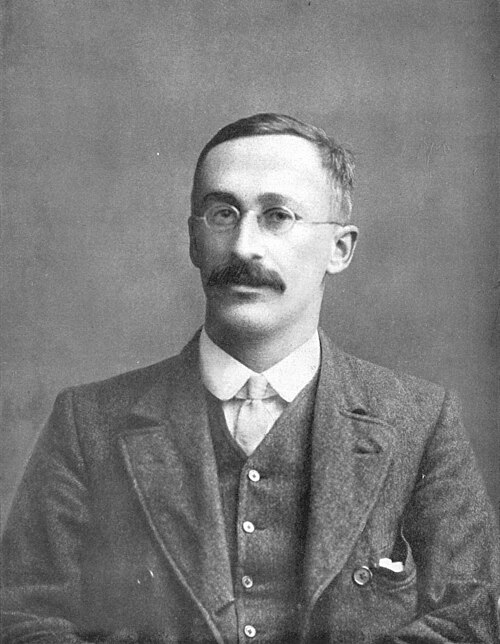
\includegraphics[width=\linewidth]{images/book3/gosset.jpg}
\end{minipage}\hfill
\begin{minipage}[t]{0.79\linewidth}
\vspace{0pt}
William Sealy Gosset, un químico que trabajaba para una cervecera, tenía que juzgar materias primas a partir de muy pocas muestras,
demasiado pocas para la ley normal. En 1908 publicó la distribución de la media dividida por la desviación típica
muestral, con el seudónimo ``Student'' porque su empresa no permitía al personal publicar
con su nombre. La ley de Student se usa cada vez que un analista da un intervalo a partir de tres o cuatro
réplicas. (Fotografía, 1908: dominio público; Wikimedia Commons.)
\end{minipage}
\end{history}

\section{Ejercicios}

\begin{exercise}[$\star$]\label{exo:b2:measurement-statistics:1}
Cinco valoraciones dan 12.45, 12.50, 12.48, 12.52 y \qty{12.46}{mL}. Calcúlense la media, la
\omterm{def:b2:measurement-statistics:dispersion}{desviación típica experimental} y la \omterm{def:b2:measurement-statistics:dispersion}{desviación típica de la media}.
\end{exercise}

\begin{exercise}[$\star$]\label{exo:b2:measurement-statistics:2}
Dese el \omterm{def:b2:measurement-statistics:confidence}{intervalo de confianza} al 95~\% de la media del ejercicio~1.
\end{exercise}

\begin{exercise}[$\star$]\label{exo:b2:measurement-statistics:3}
Se prepara una disolución disolviendo $m = \qty{0.5000}{g}$ ($u = \qty{0.0002}{g}$) de un sólido en un matraz de
$V = \qty{250.0}{mL}$ ($u = \qty{0.15}{mL}$). Calcúlese la incertidumbre típica relativa de $c = m/(MV)$,
siendo la masa molar suficientemente exacta.
\end{exercise}

\begin{exercise}[$\star$]\label{exo:b2:measurement-statistics:4}
Ajústese la \omterm{def:b2:measurement-statistics:calibration}{recta de mínimos cuadrados} que pasa por $(0, 0.02)$, $(1, 0.21)$, $(2, 0.39)$, $(3, 0.62)$.
\end{exercise}

\begin{exercise}[$\star\star$]\label{exo:b2:measurement-statistics:5}
Una disolución de referencia certificada contiene \qty{10.00}{mg/L} de un elemento. Cinco análisis dan una media de
\qty{10.12}{mg/L} con $s = \qty{0.08}{mg/L}$. ¿Está sesgado el método al nivel del 95~\%?
\end{exercise}

\begin{exercise}[$\star\star$]\label{exo:b2:measurement-statistics:6}
Una concentración de iones hidronio se conoce con una incertidumbre típica relativa del 2~\%. ¿Cuál es la
incertidumbre típica del pH?
\end{exercise}

\begin{exercise}[$\star\star$]\label{exo:b2:measurement-statistics:7}
Diez blancos tienen $s = 0.0012$ unidades de absorbancia; la pendiente de calibrado es \qty{0.0098}{L/\micro g}.
Estímense los \omterm{def:b2:measurement-statistics:limits}{límites de detección} y de cuantificación.
\end{exercise}

\begin{exercise}[$\star\star$]\label{exo:b2:measurement-statistics:8}
En el experimento de adiciones estándar de la figura, las cuatro porciones se habían preparado diluyendo
\qty{10.0}{mL} de muestra hasta \qty{50.0}{mL}. Dese la concentración en la muestra.
\end{exercise}

\begin{exercise}[$\star\star$]\label{exo:b2:measurement-statistics:9}
En un estudio interlaboratorio, cada laboratorio obtiene $s = \qty{0.05}{mg/L}$ en sus propias réplicas, pero
los resultados de los distintos laboratorios se dispersan con $s = \qty{0.15}{mg/L}$. Nómbrense las dos magnitudes y
explíquese la diferencia.
\end{exercise}

\begin{exercise}[$\star\star\star$]\label{exo:b2:measurement-statistics:10}
Demuéstrese que la \omterm{def:b2:measurement-statistics:calibration}{recta de mínimos cuadrados} pasa por $(\bar x, \bar y)$ y que sus \omterm{def:b2:measurement-statistics:calibration}{residuos} suman cero.
\end{exercise}

\begin{exercise}[$\star\star\star$]\label{exo:b2:measurement-statistics:11}
Una disolución madre se diluye cien veces, bien en una sola etapa (\qty{1.000}{mL} en \qty{100.0}{mL}), bien
en dos etapas de diez veces (\qty{10.00}{mL} en \qty{100.0}{mL}, dos veces). Incertidumbres típicas: pipeta de 1 mL
\qty{0.006}{mL}, pipeta de 10 mL \qty{0.02}{mL}, matraz de 100 mL \qty{0.08}{mL} (datos de ejercicio).
¿Qué vía es más precisa?
\end{exercise}

\begin{exercise}[$\star\star\star$]\label{exo:b2:measurement-statistics:12}
Los dos laboratorios de la introducción informan de 9.6 y \qty{11.2}{\micro g/L} con incertidumbres típicas
0.4 y \qty{0.5}{\micro g/L} (datos de ejercicio). ¿Son compatibles sus resultados? ¿Qué dice cada uno sobre el
valor guía?
\end{exercise}

\section{Problema: plomo en el agua del grifo}

\begin{problem}[{Problema de fin de semana --- un calibrado de absorción atómica por mínimos cuadrados, la
concentración de una muestra con su intervalo de confianza, la dilución y los límites, y un veredicto
frente al valor guía}]
\label{pb:b2:measurement-statistics:1}
Datos de ejercicio. El plomo se mide por absorción atómica en horno de grafito a \qty{283.3}{nm}. Patrones
(\unit{\micro g/L}; absorbancia): 0.0; 0.003, 5.0; 0.051, 10.0; 0.101, 15.0; 0.148, 20.0; 0.199. El
agua del grifo (\qty{50.0}{mL}) se acidula con \qty{0.50}{mL} de ácido nítrico; tres lecturas de esta
disolución dan 0.104, 0.098 y 0.101. Diez blancos: 0.002, 0.004, 0.003, 0.001, 0.003, 0.005, 0.002,
0.003, 0.004, 0.003. Incertidumbres típicas de los volúmenes: \qty{0.03}{mL} para 50.0 mL,
\qty{0.005}{mL} para 0.50 mL. Valor guía: \qty{10}{\micro g/L}.
% ledger: who:lead, asd:Pb283

\medskip
\noindent\textbf{Parte I --- Calibrado.}
\begin{enumerate}
  \item ¿Por qué se preparan los patrones en el mismo ácido nítrico que las muestras?
  \item Calcúlense la pendiente y la ordenada en el origen de la \omterm{def:b2:measurement-statistics:calibration}{recta de mínimos cuadrados}.
  \item Calcúlense los cinco \omterm{def:b2:measurement-statistics:calibration}{residuos}.
  \item ¿Muestran los \omterm{def:b2:measurement-statistics:calibration}{residuos} alguna tendencia? Conclúyase sobre la linealidad.
  \item Calcúlese $s_{y/x}$.
  \item ¿Por qué la ordenada en el origen no es nula?
  \item ¿Qué mide la pendiente?
\end{enumerate}

\medskip
\noindent\textbf{Parte II --- La muestra.}
\begin{enumerate}[resume]
  \item Calcúlense la media y la desviación típica de las tres lecturas.
  \item Calcúlese la concentración de plomo de la disolución medida.
  \item Calcúlese $s_{x_0}$.
  \item ¿Cuántos grados de libertad, y qué \omterm{def:b2:measurement-statistics:confidence}{coeficiente de Student}?
  \item Dese el intervalo al 95~\% de la concentración en la disolución medida.
  \item ¿Por qué leer la muestra tres veces y no una?
\end{enumerate}

\medskip
\noindent\textbf{Parte III --- Dilución y límites.}
\begin{enumerate}[resume]
  \item Calcúlense el factor de dilución y la concentración en el agua del grifo.
  \item Propáguese la incertidumbre de los dos volúmenes al factor de dilución.
  \item ¿Es significativa esa incertidumbre frente a la del calibrado?
  \item Calcúlense la desviación típica de los blancos y el \omterm{def:b2:measurement-statistics:limits}{límite de detección}.
  \item Calcúlese el \omterm{def:b2:measurement-statistics:limits}{límite de cuantificación}.
  \item ¿Está la muestra por encima del \omterm{def:b2:measurement-statistics:limits}{límite de cuantificación}?
\end{enumerate}

\medskip
\noindent\textbf{Parte IV --- Veredicto.}
\begin{enumerate}[resume]
  \item ¿Contiene el intervalo el valor guía?
  \item ¿Qué habría sugerido una sola lectura de 0.104?
  \item ¿Qué significa aquí ``confianza del 95~\%''?
  \item ¿Cómo podría el laboratorio decidir con más firmeza?
  \item ¿Cómo comprobaría que el método no está sesgado?
  \item El valor guía es provisional ``sobre la base del rendimiento del tratamiento y de la factibilidad
        analítica''. ¿Qué significa la segunda razón, a la luz de este problema?
  \item Indíquese la concentración de plomo del agua del grifo con su intervalo al 95~\%, y compárese con
        \qty{10}{\micro g/L}.
\end{enumerate}
\end{problem}
